% Source: Code/radar-scene-augmentation/architecture.tex
\documentclass[border=10pt]{standalone}
\usepackage[T1]{fontenc}
\usepackage{tikz}
\usetikzlibrary{positioning, arrows.meta}
\usepackage{helvet}
\renewcommand{\familydefault}{\sfdefault}

% Brand colors
\definecolor{garnet}{HTML}{73000A}
\definecolor{atlantic}{HTML}{466A9F}
\definecolor{congaree}{HTML}{1F414D}
\definecolor{horseshoe}{HTML}{65780B}
\definecolor{honeycomb}{HTML}{A49137}
\definecolor{grey90}{HTML}{363636}
\definecolor{grey70}{HTML}{5C5C5C}
\definecolor{grey10}{HTML}{ECECEC}

\begin{document}
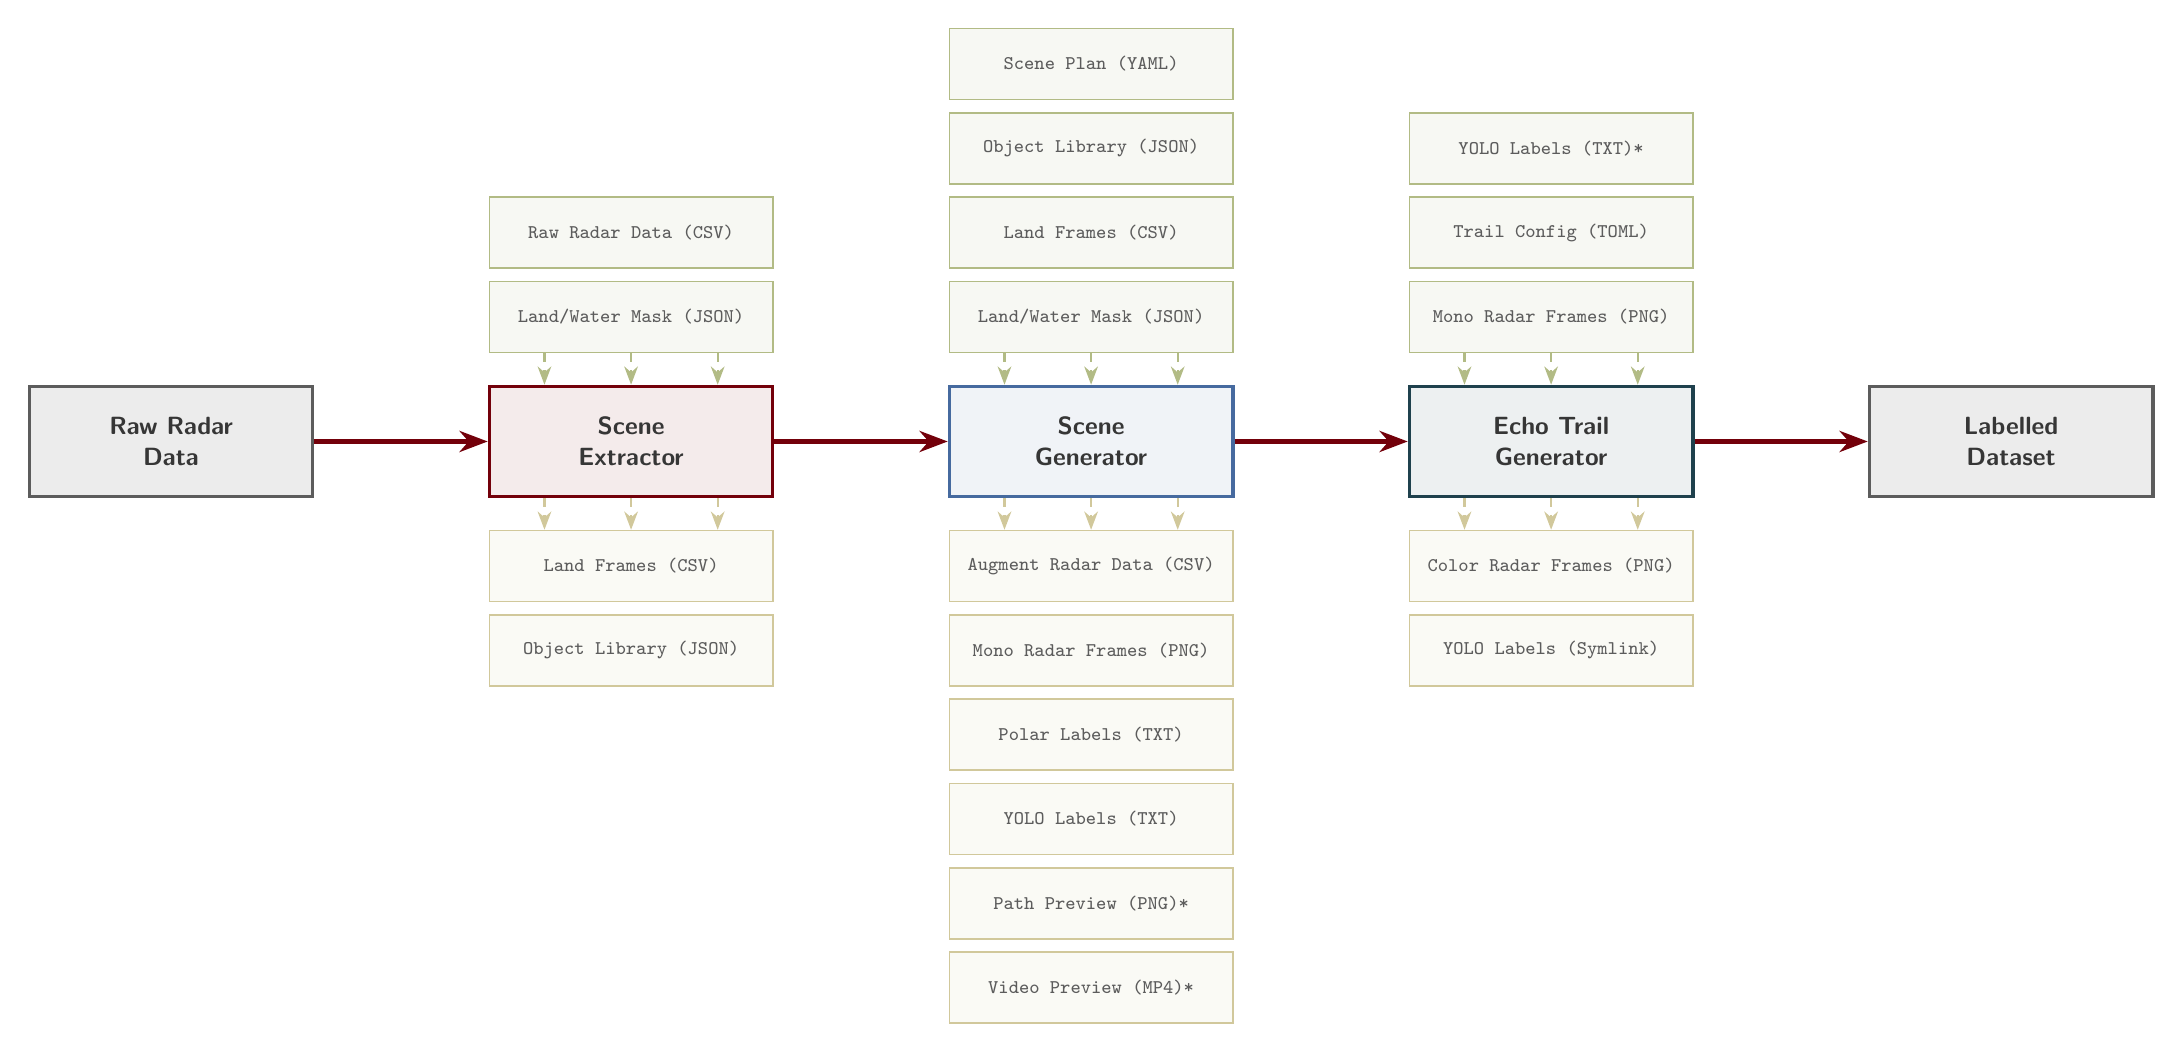
\begin{tikzpicture}[
    >=Stealth,
    pipelinebox/.style={
        rectangle,
        draw=#1,
        line width=1.2pt,
        fill=#1!8,
        minimum width=3.6cm,
        minimum height=1.4cm,
        align=center,
        font=\bfseries\small,
        text=grey90,
        inner sep=8pt,
        sharp corners,
    },
    inputbox/.style={
        rectangle,
        draw=horseshoe!50,
        line width=0.6pt,
        fill=horseshoe!5,
        minimum width=3.6cm,
        minimum height=0.9cm,
        align=center,
        font=\ttfamily\scriptsize,
        text=grey70,
        inner sep=5pt,
        sharp corners,
    },
    outputbox/.style={
        rectangle,
        draw=honeycomb!50,
        line width=0.6pt,
        fill=honeycomb!5,
        minimum width=3.6cm,
        minimum height=0.9cm,
        align=center,
        font=\ttfamily\scriptsize,
        text=grey70,
        inner sep=5pt,
        sharp corners,
    },
    iobox/.style={
        rectangle,
        draw=grey70,
        line width=1.2pt,
        fill=grey10,
        minimum width=3.6cm,
        minimum height=1.4cm,
        align=center,
        font=\bfseries\small,
        text=grey90,
        inner sep=8pt,
        sharp corners,
    },
    arrow/.style={
        ->,
        line width=1.6pt,
        color=garnet,
    },
    dashedarrow/.style={
        ->,
        line width=0.8pt,
        dashed,
        color=horseshoe!50,
    },
    dashedoutarrow/.style={
        ->,
        line width=0.8pt,
        dashed,
        color=honeycomb!50,
    },
]

% Nodes — left to right
\node[iobox]                                         (input)    {Raw Radar\\Data};
\node[pipelinebox=garnet, right=2.2cm of input]      (extract)  {Scene\\Extractor};

% Input boxes — stacked above Scene Extractor
\node[inputbox, above=0.4cm of extract]              (mask)     {Land/Water Mask (JSON)};
\node[inputbox, above=0.15cm of mask]                (rawdata)  {Raw Radar Data (CSV)};
\node[pipelinebox=atlantic, right=2.2cm of extract]  (generate) {Scene\\Generator};

% Input boxes — stacked above Scene Generator
\node[inputbox, above=0.4cm of generate]              (gen_mask)   {Land/Water Mask (JSON)};
\node[inputbox, above=0.15cm of gen_mask]             (gen_land)   {Land Frames (CSV)};
\node[inputbox, above=0.15cm of gen_land]             (gen_objlib) {Object Library (JSON)};
\node[inputbox, above=0.15cm of gen_objlib]           (gen_scene)  {Scene Plan (YAML)};
\node[pipelinebox=congaree, right=2.2cm of generate] (trail)    {Echo Trail\\Generator};

% Input boxes — stacked above Echo Trail Generator
\node[inputbox, above=0.4cm of trail]                (trail_frames) {Mono Radar Frames (PNG)};
\node[inputbox, above=0.15cm of trail_frames]        (trail_config) {Trail Config (TOML)};
\node[inputbox, above=0.15cm of trail_config]        (trail_labels) {YOLO Labels (TXT)*};

\node[iobox,               right=2.2cm of trail]    (output)   {Labelled\\Dataset};

% Output boxes — stacked below Scene Extractor
\node[outputbox, below=0.4cm of extract]             (landframes) {Land Frames (CSV)};
\node[outputbox, below=0.15cm of landframes]         (objlib)     {Object Library (JSON)};

% Output boxes — stacked below Scene Generator
\node[outputbox, below=0.4cm of generate]            (gen_csv)    {Augment Radar Data (CSV)};
\node[outputbox, below=0.15cm of gen_csv]            (gen_png)    {Mono Radar Frames (PNG)};
\node[outputbox, below=0.15cm of gen_png]            (gen_raw)    {Polar Labels (TXT)};
\node[outputbox, below=0.15cm of gen_raw]            (gen_yolo)   {YOLO Labels (TXT)};
\node[outputbox, below=0.15cm of gen_yolo]           (gen_path)   {Path Preview (PNG)*};
\node[outputbox, below=0.15cm of gen_path]           (gen_video)  {Video Preview (MP4)*};

% Output boxes — stacked below Echo Trail Generator
\node[outputbox, below=0.4cm of trail]               (trail_out_frames) {Color Radar Frames (PNG)};
\node[outputbox, below=0.15cm of trail_out_frames]   (trail_out_labels) {YOLO Labels (Symlink)};

% Dashed arrows from Echo Trail Generator to outputs at 1/4, 1/2, 3/4 marks
\draw[dashedoutarrow] ([xshift=-1.1cm]trail.south) -- ([xshift=-1.1cm]trail_out_frames.north);
\draw[dashedoutarrow] (trail.south)                -- (trail_out_frames.north);
\draw[dashedoutarrow] ([xshift=1.1cm]trail.south)  -- ([xshift=1.1cm]trail_out_frames.north);

% Dashed arrows from inputs to Echo Trail Generator at 1/4, 1/2, 3/4 marks
\draw[dashedarrow] ([xshift=-1.1cm]trail_frames.south) -- ([xshift=-1.1cm]trail.north);
\draw[dashedarrow] (trail_frames.south)                -- (trail.north);
\draw[dashedarrow] ([xshift=1.1cm]trail_frames.south)  -- ([xshift=1.1cm]trail.north);

% Dashed arrows from Scene Extractor to outputs at 1/4, 1/2, 3/4 marks
\draw[dashedoutarrow] ([xshift=-1.1cm]extract.south) -- ([xshift=-1.1cm]landframes.north);
\draw[dashedoutarrow] (extract.south)                -- (landframes.north);
\draw[dashedoutarrow] ([xshift=1.1cm]extract.south)  -- ([xshift=1.1cm]landframes.north);

% Dashed arrows from Scene Generator to outputs at 1/4, 1/2, 3/4 marks
\draw[dashedoutarrow] ([xshift=-1.1cm]generate.south) -- ([xshift=-1.1cm]gen_csv.north);
\draw[dashedoutarrow] (generate.south)                -- (gen_csv.north);
\draw[dashedoutarrow] ([xshift=1.1cm]generate.south)  -- ([xshift=1.1cm]gen_csv.north);

% Dashed arrows from inputs to Scene Generator at 1/4, 1/2, 3/4 marks
\draw[dashedarrow] ([xshift=-1.1cm]gen_mask.south) -- ([xshift=-1.1cm]generate.north);
\draw[dashedarrow] (gen_mask.south)                -- (generate.north);
\draw[dashedarrow] ([xshift=1.1cm]gen_mask.south)  -- ([xshift=1.1cm]generate.north);

% Dashed arrows from mask to Scene Extractor at 1/4, 1/2, 3/4 marks
\draw[dashedarrow] ([xshift=-1.1cm]mask.south) -- ([xshift=-1.1cm]extract.north);
\draw[dashedarrow] (mask.south)                -- (extract.north);
\draw[dashedarrow] ([xshift=1.1cm]mask.south)  -- ([xshift=1.1cm]extract.north);

% Pipeline arrows
\draw[arrow] (input)    -- (extract);
\draw[arrow] (extract)  -- (generate);
\draw[arrow] (generate) -- (trail);
\draw[arrow] (trail)    -- (output);

\end{tikzpicture}
\end{document}
